\chapter[The Volcanic History of Syria Planum, Mars]{
The Volcanic History of Syria Planum, Mars \footnote{This chapter has been reprinted from the Journal of Volcanology and Geothermal Research with permission from XXX as: Richardson, J. A., Bleacher, J. E., Glaze, L. S., (2013), The Volcanic History of Syria Planum, Mars, Journal of Volcanology and Geothermal Research, 252, 1-13.}}\label{ch_syria}

\renewcommand*{\FigPath}{figures/chapter-syria_planum}

\section{Abstract}
A field of small (10s~km in diameter) volcanoes in the Syria Planum region of Mars is mapped to determine abundance, distribution, and alignments of vents.  These data are used to assess possible variations in eruption style across space and time. Each eruption site is assigned a point location. Nearest neighbor and two--point azimuth analyses are conducted to assess the spacing and orientations between vents across the study area. Two vent fields are identified as unique volcanic units along with the previously identified Syria Mons volcano.  Superposition relationships and crater counts indicate that these three volcanic episodes span $\sim$900 Ma, beginning in the early Hesperian and ending in the Early Amazonian. No clear hiatus in eruptive activity is identified between these events, although a progression from eruptions at Syria Mons, to regionally distributed eruptions that form the bulk of the Syria Planum plains, to a final migration of dispersed eruptions to Syria's northwest is identified. Nearest neighbor analyses suggest a non--random distribution among the entire population of Syria Planum, which is interpreted as resulting from the interaction of independent magma bodies ascending through the crust during different stress regimes throughout the region's eruptive history. Two--point azimuth results identify three orientations of enhanced alignments, which match well with radial extensions of three major tectonic centers to the south, east, and northwest of the study area. As such, Syria Planum volcanism evolved from a central vent volcano to dispersed shield field development over several hundred million years, during which the independent magma bodies related to each small volcano interacted to some extent with one or more of at least three buried tectonic patterns in the older crust.  These results show a strong relationship between independent mapping efforts of tectonic and volcanic features. Continued integration of volcano--tectonic mapping should provide direct constraints for future geodynamic models of magma production and thermal evolution of the Tharsis province.

\section{Introduction}
\label{sec-intro}

The Tharsis province is a volcanic rise extending over 4500 km across the western hemisphere of Mars, covering nearly a quarter of the planet's surface \citep{Hodges1994}. This region is suggested to display volcanic and tectonic activity into the late Amazonian \citep{Anderson2001,neukum2004recent} (Martian chronology is detailed briefly in Section \ref{sec:methodCrater}). The region is long recognized to include five major shield volcanoes, seven partly buried volcanoes, vast lava plains, and a wide range of smaller eruptive vents \citep{carr1977some,Greeley1981,MouginisMark1992,Hodges1994}. While twelve large named volcanoes are cataloged and their morphologies and morphometries described in detail \citep[][and references therein]{Hodges1994,plescia2004morphometric}, small volcanic edifices (10s km in diameter) have received much less attention due to a lack of high resolution data with regional coverage prior to the Mars Global Surveyor (MGS) mission.

The acquisition of post--\textit{Viking} data enables for the first time detailed cataloging and morphologic descriptions of the wide range of small volcanic vents (hereafter referred to as small vents) in the Tharsis province \citep{baptista2008swarm,Baratoux2009,bleacher2007tharsis,bleacher2009spatial,Broz2012,Hauber2009,hauber2011very,Keszthelyi2008,Wilson2009}. This ability represents a critical step forward in the scientific understanding of Martian magma production and eruption. Because different types of volcanic features result from a combination of different eruptive conditions, magma and lava properties, and ambient variables \citep{greeley1977basaltic,WhitfordStark1982}, an understanding of the abundance and distribution of volcanic features serves as a fundamental framework that is needed to fully understand any volcanic system \citep{Head1981,Connor2000}.

Here we report on mapping and analyses of the vent fields within the Syria Planum region of Mars \citep{baptista2008swarm}. This is a portion of an ongoing investigation to catalog the location of small (10s km in diameter) vents across the Tharsis region.  Although each vent appears minor in areal coverage and volume compared to the larger Tharsis shield volcanoes, when considered together as vent fields comparable to the Snake River Plain in Idaho, USA \citep{greeley1977basaltic,Greeley1982}, they represent significant magma production events. In addition to the volume of lava visible on the surface, the entire crust of the Tharsis region appears to have been demagnetized \citep{Connerney2005,Lillis2006}. The passage of many small magma packages into and through the crust provides a plausible explanation for this demagnetization in areas that are hundreds of kilometers away from major shield volcanoes \citep{Lillis2009}.  Likewise, tectonic evidence has led to the suggestion that the Tharsis province has experienced multiple episodes of large mantle upwellings \citep{Plescia1982,mege1996plume,Anderson2001,Anderson2004,Wilson2002}, the centers of which are not necessarily spatially overlapping with major volcanoes.  \citet{Anderson2001,Anderson2004} refer to these events as magmatic-driven tectonic episodes, which is consistent with the identification of vent fields in the Tharsis plains.  As such, it is critical to assess the number, location, and duration of magma production events that contributed to the current morphology of the Tharsis region.

\subsection{Geologic Description}

Past mapping of Syria Planum has enabled the identification of several distinct units based on morphologic characteristics. \citet{baptista2008swarm} identified three distinct units in southwestern Syria: 1) a unit comprised of NW--trending graben, 2) lava flows associated with Syria Mons, and 3) a field of coalesced low shield volcanoes. The lava flows associated with Syria Mons are hundreds of kilometers in length and form kilometers--wide, finger--like sheets of lava throughout the unit. These flows embay the graben field, which is composed of narrow (100s of meters to kilometers) linear and curvilinear graben that are tens to hundreds of kilometers in length. The Syria Mons flows are crosscut by NE--SW trending graben, 10s of km in length. The coalesced shield field is composed of low shield volcanoes several kilometers in diameter that embay the Syria Mons lava flows. Both the field and the flows are crosscut with NW--SE trending graben (km in length). A newly identified geologic unit (Hnsf in Figure \ref{fig-geomap}) is located to the north of the \citet{baptista2008swarm} study area and is seen to embay the coalesced shield field to the south. It is characterized by lava flows tens to hundreds of kilometers in length emanating from a topographic ridge approximately 200km in length that trends NE--SW. The lava flows that form this unit are seen to fill preexisting graben that crosscut the southern coalesced shield field and embay vents from the southern shield field.

\begin{figure}
	\centering
	\includegraphics[width=0.8\linewidth]{\FigPath/fig1.eps}
	\caption[Geologic Map of Syria Planum]{Geologic Map of Syria Planum. The study area is shown inside the thick black line with a MOLA-derived hillshade basemap. The study area of \citet{baptista2008swarm} is shown as a rectangle in the south--central region of the study area. In the east a dotted line surrounds an area where no volcanic vents are found and is therefore not included in the study area (crater counting was not performed in this area). Volcanic vents are represented as a solid black point, likely volcanic vents as a white point outlined in black, and Syria Mons is represented as a star. Graben are shown as thin black lines. White lines separate geologic units. From north to south these units are: Hp, a unit on the margins of the plateau that features scattered individual vents; Hnsf, a northern shield field of coalesced volcanic vents; Hssf, a southern shield field of coalesced volcanic vents; Hsm, lava flows of Syria Mons; Hg, a graben-rich unit; Hlp, a unit of lava flows on the southeast margin of Syria Planum that hosts relatively few volcanic vents.}
	\label{fig-geomap}
\end{figure}

The mapping of \citet{baptista2008swarm} was limited by High Resolution Stereo Camera (HRSC) data availability to 100-105$^{\circ}$W, 13-23$^{\circ}$S within the Syria region. Despite this limitation, \citet{baptista2008swarm} demonstrated that analysis of high resolution image data with regional coverage showed new volcanic and tectonic complexities in this region that had previously been identified as a plains style volcanic province \citep{Sakimoto2003} similar to those described on the Earth \citep{Greeley1982}, and other Mars volcanic field studies \citep{bleacher2007tharsis,bleacher2009spatial,Hauber2009}. The addition of several tectonic episodes that temporally separate volcanic emplacement events leads to the hypothesis that Syria Planum is the surface product of multiple (opposed to one long--lived) magma production events. For clarity, we use the term ``magma production event'' to represent a broad magmatic upwelling that might feed multiple shallow, crustal magma bodies and small volcanic vents across a region like Syria. Such an event might be comparable to an event that feeds a major shield like Olympus Mons or each of the Tharsis Montes, and should be considered in models of the thermal and geologic evolution of Tharsis. Therefore, it is imperative to determine if a large field of vents like Syria represents one magma production event, or possibly multiple, temporally distinct events that are spatially overlapping on the surface of the planet.

In order to test this hypothesis we map volcanic vents in the full Syria Planum region at comparable resolutions to the study of \citet{baptista2008swarm}, which is only now possible due to the combined data acquisition of HRSC, Thermal Emission Imaging System (THEMIS), and Context Imager (CTX) images. Our objectives are to determine if multiple separable magma production events occurred in Syria and to assess whether these events can be clearly identified as unique events or the extension of a long--lived, continuous magma production event, either of which provide new insight into and modeling constraints for the thermal and tectonic evolution of the Tharsis province.

In this paper, new spatio--temporal boundaries of known volcanic units are presented and a new volcanic unit in the north of Syria is identified, separated from southern volcanism by a distinct flow margin. Each volcanic unit in Syria Planum is temporally constrained with superposition relationships and crater age--dating. Methods which are used to spatially describe small volcanic vents in Syria are then discussed, including nearest neighbor and 2--point azimuth statistical analyses. Finally, a revised volcano--tectonic history of Syria Planum is proposed, wherein we interpret that volcanism has likely migrated spatially throughout the evolution of Syria and wherein the style of volcanism has likely shifted from one central vent at Syria Mons to forming coalesced shield fields.

\section{Methods}

\subsection{Study Area}

The study area (Figure \ref{fig-geomap}), Syria Planum, is located on the southeastern margin of the Tharsis province between 8-23$^{\circ}$S and 110-93$^{\circ}$W. Syria Planum is bordered by Noctis Labyrinthus to the north, Claritas Fossae to the west and Solis Planum to the southeast. This area forms a regional plateau with a maximum elevation of 8000 m based on analysis of Mars Orbiter Laser Altimeter (MOLA) \citep{smith2003mars} gridded data. A total relief of 4000 m exists between this point and the southeastern portion of the study area. The study area is roughly 1000 by 900 km in size as defined by \citet{Scott1986}, with an abundance of volcanic vents focused in an area roughly 700 by 600 km in size \citep{Richardson2010,Richardson2012}. In order to characterize the volcanic evolution of Syria all identifiable volcanic vents in the study area are mapped and morphologic units are identified as temporally separable by crater counting. Nearest neighbor and 2--point azimuth statistical analyses are applied to the vent location data to provide additional constraints on the evolution of the volcanic region. A 512 pixels--per--degree (ppd) THEMIS infrared (IR) day--time mosaic \citep{Christensen2004} and the 128 ppd MOLA gridded dataset \citep{smith2003mars} are used as base maps. Relevant CTX \citep{malin2007context} and THEMIS visible (VIS) \citep{Christensen2004} images are co-registered to this base map for the identification of volcanic vents.

\subsection{Catalog of Volcanic Vents}

Volcanic vents are spatially cataloged as single points in a Cartesian grid, referencing their plan view position with respect to the THEMIS IR day--time mosaic and the gridded MOLA dataset base maps. Each datum is assumed to closely represent the four--dimensional (space and time) pathway along which magma ascended through the crust to erupt at the surface and produce an identifiable vent structure \citep{Bishop2007}. Volcanic vents are here defined as positive topographic landforms, tens to hundreds of meters in height, with flows or flow--like textures radiating from the apex and/or depressions at the topographic summit. Many positive topographic landforms lack clear flow features or a preserved depression at the apex, but are otherwise morphologically similar to cataloged vents. These landforms, which are tens to hundreds of meters in height, are also cataloged as likely volcanic vents (an example with contours is shown in Figure \ref{fig-geomap}). It is assumed that many volcanic vents that formed within the volcanic field on Syria Planum have since been buried by continued volcanism. This mapping project does not consider these buried vents, nor does this study provide any assumptions about stalled magma bodies for which ascension pathways were established but did not lead to surface eruptions (in other words, the intrusion to extrusion ratio of the region as was estimated in southern Tharsis by \citet{Lillis2009}). Instead, vents that are currently identifiable on the surface are assumed to represent the last stage of eruptive activity in the region and are used to provide new insight into the magmatic and volcanic history of Syria and the Tharsis province.

A variety of volcanic vent morphologies are present on Tharsis and have recently been characterized using post--\textit{Viking} era image data \citep{bleacher2007tharsis,bleacher2009spatial,Broz2012,Keszthelyi2008,baptista2008swarm,Hauber2009,Wilson2009,Baratoux2009}. Different methods are implemented for different vent morphologies to realistically assign a representative two--dimensional point to this four--dimensional process. For volcanic vents with depressions at the summit from which lava has visibly erupted (based on interpretation of radiating textures or buildup of spatter or cinder rims (examples in Figure \ref{fig-geomap})) a data point is digitally created  at the center of the depression using ArcGIS 9.3. For volcanic vents with linear depressions along a topographic high, the data point is created at the midpoint of a line with endpoints at the extents of the depression. In cases where the depression extends beyond the apparent eruptive activity (in other words, an extended dry fracture associated with the eruptive segment of the fissure as discussed by \citet{greeley1977basaltic} in volcanic fields) the data point is assigned at the middle point of a line connecting the ends of the eruptive segment. For likely volcanic features, which do not display summit depressions, data points were assigned at the topographic summit of the feature or at the origin of radiating flow textures where possible.

Cataloging the location of volcanic vents within Syria also enables the identification of distinct large scale flow features and units based on different morphological and superposition characteristics.  Consistent superposition relationships among vent groups within Syria are identified. Using the map of vent locations (Figure \ref{fig-geomap}) and superposition relationships for Syria Planum, several techniques are applied to further characterize the region's eruptive history. Based on the identification of unique vent groups, crater counts (described in Section \ref{sec:methodCrater}) are conducted to test whether quantifiable hiatuses occurred between the formation of different volcanic and tectonic events. Nearest neighbor analysis (described in Section \ref{sec:methodNN}) is applied to the complete Syria vent catalog and to subgroups of vents within the study area based on morphological mapping units. Nearest neighbor analysis is applied to assess the spatial distribution among vents. This has been shown as a method of characterizing a group of data points as being composed of one or a combination of populations \citep{Bishop2007, Baloga2007}. A two--point azimuth technique (described in Section \ref{sec:methodAzimuth}) is implemented to identify potential lineaments between volcanic vents that might correlate to underlying structures \citep{Lutz1986,Wadge1988,Wadge1989,connor1990cinder,lutz1995improved,bleacher2009spatial} in an attempt to better understand the ascent of magma beneath Syria. The combination of such spatial and alignment analyses has been used to characterize volcanic fields on the Earth \citep{Lutz1986,lutz1995improved,Cebria2011,Roberts2011} and Mars \citep{bleacher2009spatial}.

\subsection{Crater Counting}
\label{sec:methodCrater}

Using the 512ppd THEMIS infrared daytime mosaic, craters larger than 0.5~km in diameter are cataloged in accordance with identified vent groups and morphologic units. For each morphologic unit, a crater retention age is fitted to a cumulative crater size--frequency distribution following the method described in \citet{hartmann2005martian} and using the freely available software Craterstats2 \citep{Michael2010}. The size--frequency distribution is fit to a production function from \citet{Ivanov2001} and an absolute age is calculated using the chronology model from \citet{Hartmann2001}.

Given the relatively large surface area of each morphologic unit (e.g. one unit is composed of $>$100 volcanic shields) and the relatively low spatial resolution of the THEMIS mosaic (100~m), isochrons for this study are fit using craters of diameter $\ge$1~km. Craters of diameter $<$1~km are not used for determining ages due to the tendency for the number of smaller craters to artificially diminish as their diameter approaches the resolution of the base map.s Crater retention rates are reported with errors following the equation
\begin{equation}
N(1) = \frac{n_{1km}}{A} \pm \frac{\sqrt{n_{1km}}}{A} \label{eq1}
\end{equation} 
where $n_{1km}$ is the observed number of craters with diameters greater than 1 km and $A$ is the surface area in km$^2$.

Ages determined by crater age--dating are assigned an epoch range based on the Martian chronostratigraphic system as recently outlined by \citet{Werner2011}. Generally, the three periods of the Martian system are the Noachian, Hesperian, and Amazonian, ranging from $>$3.96-3.57~Ga, 3.57-3.00~Ga, and 3.00~Ga-present, based on the chronology model of \citet{hartmann2005martian}, respectively. These periods are further separated into epochs as follows: Middle Noachian, 3.96-3.85~Ga; Late Noachian, 3.85-3.57~Ga; Early Hesperian, 3.57-3.40~Ga; Late Hesperian, 3.40-3.00~Ga; Early Amazonian, 3.00-0.88~Ga; Middle Amazonian, 0.88-0.24~Ga; Late Amazonian, 0.24~Ga to present.

\subsection{Nearest Neighbor Analysis}
\label{sec:methodNN}

The distances from each volcanic vent to its nearest neighboring vent in a volcanic field can be used to characterize the spatial distribution of the volcanic vents within a field. It has been hypothesized that the vents of a terrestrial volcanic vent field (i.e. field volcanism) will conform to a random spatial distribution \citep{Lutz1986,lutz1995improved}. This is to say that each vent is located in the study area independently of the location of any other vent, that each vent has the same probability of occurrence at any location in the study area, and that any subarea of the study area is equally likely to contain any vent as any other identically sized study area \citep{Clark1954}.

Based on the Poisson spatial distribution, \citet{Clark1954} defined two statistics with which to analyze nearest neighbor (NN) distances for a spatial distribution of points. First, the test statistic, $c$, is given by the equation 
\begin{equation}
c= \frac{\bar{r}_a -\bar{r}_e}{\sigma_e},  \label{eq3}
\end{equation}
where $\bar{r}_a$ is the mean observed NN distance, $\bar{r}_e$ is the expected mean NN distance for a Poisson spatial distribution, and $\sigma_e$ is the expected standard deviation of NN distances. Expected values of $c$ were simulated by \citet{Baloga2007} to remove bias based on sample size. If the observed $c$ statistic departs from the expected $c$ by more than $2\sigma$ for the appropriate sample size, spatial randomness may be rejected.

Second, the ratio between the observed mean NN distance, $\bar{r}_a$, and the expected mean NN distance, $\bar{r}_e$, given by equation \ref{eq4}, also tests the fit of Poisson randomness.
\begin{equation}
R = \frac{\bar{r}_a}{\bar{r}_e} \label{eq4}
\end{equation}
If a vent field is spatially random in a Poisson sense, the $R$-index will approach 1. Values of $R~>$~1 suggest that the points approach maximal packing, while values of $R~<$~1 suggest that points are more clustered than expected for a Poisson spatial distribution. Similar to the test statistic $c$, the calculated $R$--index may be compared to an expected $R~\pm~2\sigma$ to test for the fit of Poisson randomness to describe the distribution of points.

\citet{Baloga2007} also developed a test using the skewness and kurtosis of the NN distribution to further constrain the applicability of the Poisson distribution to a spatial sample. Using 1000 simulated Poisson point sets of the same sample size, it was observed that skewness and kurtosis are strongly correlated and focus around an elliptical centroid.  If the skewness and kurtosis values for a given point set plot sufficiently far away from the centroid of simulated Poisson values, randomness in the Poisson sense may again be rejected.

Nearest neighbor analysis described above can be used to quantitatively compare the spatial distribution of volcanic vents with the null hypothesis, H$_o$, of spatial randomness in a Poisson sense. We hypothesize that if the vents are spatially random in the Poisson sense, then the vents have formed independently of each other as part of one larger magma production event (e. g. their respective magma ascension pathway through the crust was not influenced by the location of any other vent thereby causing a random spacing of eruption points). If a Poisson distribution is rejected and the $R$--index statistic shows evidence for clustering, we interpret the result as evidence that multiple temporally distinct magma production events have occurred beneath Syria Planum that are spatially overlapping, thereby resulting in two or more random but mixed statistical populations \citep{Lutz1986,lutz1995improved}.

To perform nearest neighbor analysis, Geological Image Analysis Software (GIAS), version 1.12, was used \citep{Beggan2010,Hamilton2010,Hamilton2011}.

\subsection{Two--point azimuthal analysis}
\label{sec:methodAzimuth}

Two--point azimuth techniques have been used to observe and describe lineaments between volcanic vents for decades \citep{Lutz1986,Wadge1988,Wadge1989,connor1990cinder,lutz1995improved,bleacher2009spatial,Cebria2011,Roberts2011}. Azimuth techniques determine the directions from each point to every other point. Lineaments between vents are identified by looking at anomalously high numbers of azimuths in any given direction and comparing that with other linear features, such as faults and graben, observed in the area or in adjacent, older terrains for which their traces might have been buried by the emplacement of the volcanic field or other geologic processes.

\citet{Cebria2011} postulated that lineaments between two vents are more likely if those vents are relatively close to each other. They therefore suggested that two point azimuth techniques should use a \textit{minimum significant distance}, a distance where the azimuths of closer inter--vent relationships best characterize lineaments of the given field. Inter--vent relationships farther than this minimum significant distance are not as likely to be related by the same underlying geological structures. Adding to the benefit of using only inter--vent relationships smaller than this distance is that anomalously far inter--vent relationships will likely display bias in the direction of the vent field's major axis. If the vent distribution for example, resembles a narrow ellipse due to topographic focusing, the longer inter--vent relationships will necessarily point in the direction of the long axis of the ellipse even if regional tectonic patterns are perpendicular.

For this study, the minimum significant distance used is defined by \citet{Cebria2011}
\begin{equation}
d \le (\mu_v - 1\sigma_v) / 3 \label{eq5}
\end{equation}
where $\mu_v$ is the mean inter--vent distance and $\sigma_v$ is the standard deviation of inter--vent distances. Using the set of inter--vent relationships shorter than this distance, relationships are grouped by direction into nine bins of a rose diagram. We hypothesize that bins containing an anomalous amount (count~$\ge~\bar{x}_n~+~\sigma_n$) of inter--vent relationships are evidence of lineaments between vents. These orientations are compared with regional tectonic trends as possible influences of magma ascension \citep{bleacher2009spatial,Cebria2011}.

\section{Results}

\subsection{Mapping}

In the study area 263 vents are identified, with 206 cataloged as volcanic vents and 57 cataloged as likely volcanic vents. There is no specific area where likely volcanic vents (as opposed to volcanic vents) are concentrated, though the highest abundance of likely volcanic vents are in northern Syria Planum. Because of the likely volcanic vents' regional distribution and topographic similarity to landforms cataloged as volcanic vents, we have included likely volcanic vents in the statistical analysis of all volcanic vents on Syria Planum. Here after both categories of vents are treated as one catalog, which includes 263 features.

The 263 identifiable vents within Syria Planum are distributed among five of six identified map units on Syria, which are delineated based on observed superposition relationships. Cataloged volcanic vents, geologic units, and graben are plotted in Figure \ref{fig-geomap}. A graben--rich unit previously described by \citet{baptista2008swarm} and \citet{Tanaka1988}, Hg, is located in the southwest of the study area and is seen to be embayed by the lavas of the Syria Mons unit, Hsm. Lavas associated with Syria Mons cover much of the study area and extend at least several hundreds of kilometers from Syria Mons' main vent towards the southeast. The Syria Mons summit is the only vent cataloged in this unit. The boundaries of the Syria Mons unit are defined to the west and south by the margins of distinct, overlying lava flows. To the east, the Syria Mons unit is embayed by low shields that coalesce into a volcanic vent field, Hssf. Syria Mons and thirty volcanoes that make up this coalesced vent field unit were extensively mapped by \citet{baptista2008swarm}. The majority of vents cataloged in Syria Planum, 192, are cataloged in this vent field. Low shields that coalesce to form this unit have slopes 1-2.5$^{\circ}$ and diameters between 10 and 35 kilometers. Eight vents are identified in this unit that have slopes up to 6$^{\circ}$ and diameters of 2-10~km. The low shields of this unit extend into the southeast where they flow over a unit of large scale lava flows, Hlp, that extend from a center within Syria Planum, which is unrecognized at this time. In this southeastern unit, 6 vents are cataloged.

To the north of the coalesced unit are distinct flow margins. The lava that created these flow margins embay low shields associated with the coalesced unit and fill graben that have cross--cut the coalesced unit. The source of the embaying lava flows to the north is a unit comprised of 22 vents that form a second coalesced volcanic vent field. To distinguish between these two coalesced volcanic units, the field to the south, Hssf, is labeled as the ``southern shield field'' and the field to the north, Hnsf as the ``northern shield field.'' The northwestern boundary of the northern shield field is determined by the extent of visible lava flows, which extend to the north and south of the vents as far as 200~km. The northwest region of the study area is identified as one unit, Hp, beyond the lava flows of Syria Mons and the northern shield field. The northwestern unit contains 42 vents, which do not coalesce together to make one distinct field. The relative superposition of this unit to the Syria Mons lava flows and the northern shield field are not clearly defined.

\begin{table}
\centering
\caption{Summary of Vent Counts in Defined Units}
\label{tab-ventct}
\begin{tabular}{l c c c}
\toprule
& Volcanic Vents & Likely Volcanic Vents & Total Vents  \\
\midrule
Northern Shield Field, \textit{Hnsf}$^*$ & 13 & 9 & 22 \\
Southern Shield Field, \textit{Hssf}$^*$ & 159 & 33 & 192 \\
Syria Mons Unit, \textit{Hsm} & 1 & 0 & 1 \\
Northwest Syria Planum, \textit{Hp} & 28 & 14 & 42 \\
Southeast Syria Planum, \textit{Hlp} & 4 & 2 & 6 \\
\midrule
Totals & 205 & 58 & 263 \\
\bottomrule
\multicolumn{4}{p{0.95\linewidth}}{$^*$Nearest neighbor analysis is performed on the vent populations of the northern and southern shield fields and the combination of these fields.}
\end{tabular}
\end{table}


The vents of the two coalesced shield fields are identified as subgroups within the catalog of Syria Planum vents and are used for statistical analysis in this study. The locations of volcanic vents cataloged in the study area are summarized in Table \ref{tab-ventct}. Because the flow fronts farthest from, but still associated with, the northern shield field are buried by successive flow fronts closer to the observed vents of the shield field, their temporal connection to the observed vents is not confirmable. For this reason, geologically lower flow fronts which are embayed by flows and are not able to be connected to northern shield field vents are described as intermediate flows in age--dating exercises discussed in Section \ref{sec:resultsAgeDating}.

\subsection{Age--Dating}
\label{sec:resultsAgeDating}

\begin{table}
\centering
\caption{Crater Retention Rates and Ages for Selected Units}
\label{tab-crater}
\begin{tabular}{l c c l}
	\toprule
  & 10$^{-3}$~N(1) & Age, & Epoch$^*$\\
  & craters~km$^{-2}$ & Ga &\\
  \midrule
  Northern Shield Field, \textit{Hnsf} & 1.4$\pm$0.2 & 2.56-3.23 & Late Hesp. to Early Amaz. \\
  Northwest Syria Planum, \textit{Hp} & 1.5$\pm$0.1 & 3.17-3.29 & Late Hesp. \\
  Intermediate Flows, \textit{Hnsf?} & 1.7$\pm$0.4 & 3.28-3.52 & Early to Late Hesp. \\
  Southern Shield Field, \textit{Hssf} & 1.7$\pm$0.1 & 3.23-3.35 & Late Hesp. \\
  Southeast Syria Planum, \textit{Hlp} & 1.8$\pm$0.1 & 3.33-3.40 & Late Hesp. \\
  Syria Mons Unit, \textit{Hsm} & 2.0$\pm$0.1 & 3.41-3.47 & Early Hesp. \\
  Graben Basement, \textit{Hg} & 2.2$\pm$0.2 & 3.37-3.46 & Early to Late Hesp.\\
	\bottomrule
	\multicolumn{4}{p{0.95\linewidth}}{$^*$Hesp.: Hesperian; Amaz.: Amazonian.}
\end{tabular}
\end{table}

In Table \ref{tab-crater} and illustrated graphically in Figure \ref{fig-unitages}, crater counts and their corresponding age-dates are presented. According to these counts, the last lava flowed over the surface of Syria Planum as recent as the early Amazonian. Crater dating also shows that the lavas from Syria Mons and the graben--rich basement that they embay, which are the lowest observed geologic units, were last significantly resurfaced during the early Hesperian epoch.

\begin{figure}
\centering

\includegraphics[width=0.7\linewidth]{\FigPath/fig2.eps}
\caption{Graphical summary of age--dating results by unit.}
\label{fig-unitages}
\end{figure}

Using superposition, volcanic units are relatively dated with Syria Mons erupting first, low shields of the southern shield field embaying its flows, and lavas of the northern shield field embaying the southern shield field. As shown in Figure \ref{fig-unitages}, error bars between ages of flows associated with Syria Mons, the southern shield field, and the northern shield field do not overlap and are in agreement with superposition observations. However, no significant haitus exists between the development of each unit. While some units seem ambiguously dated with respect to superposition (e.g. the graben--rich basement unit upon which are flows from Syria Mons is dated to be younger than the Syria Mons flows), no unit is in direct disagreement with relative dating observations, within error.

\subsection{Nearest Neighbor Analysis}

\begin{figure}
\centering
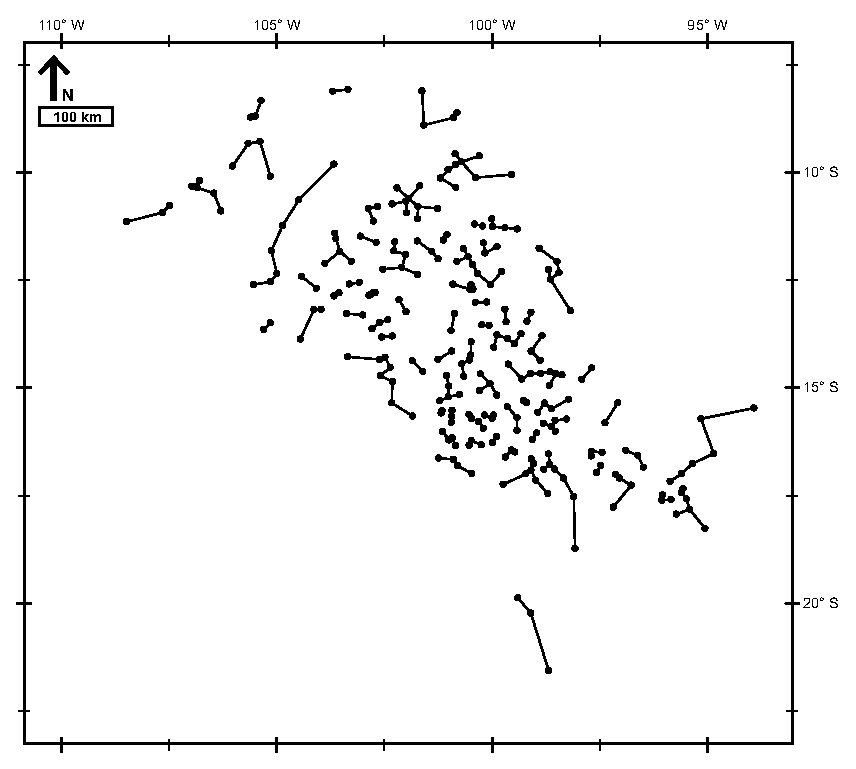
\includegraphics[width=0.5\linewidth]{\FigPath/fig3.eps}
\caption{Plot of vents with lines drawn to their nearest neighbors.}
\label{fig-nnmap}
\end{figure}

Figure \ref{fig-nnmap} is a map of all vents cataloged in Syria Planum with lines drawn to represent the connections from each vent to their nearest neighbor. Nearest neighbor analysis is conducted using these distances. Table \ref{tab-nn} presents results of the nearest neighbor analyses. The first two columns of Table \ref{tab-nn} give the expected and observed nearest neighbor distances for each area examined. The columns for $R_e$ and $c_e$ give the acceptance ranges for values of $R$ (defined in Equation \ref{eq4}) and $c$ (defined in Equation \ref{eq3}), respectively, based on sample size. The results of the skewness/kurtosis test are plotted in Figure \ref{fig-skgraphs}. Each plot shows simulated values of skewness and kurtosis for 1000 random Poisson spatial distributions (in gray). When the black diamond (indicating observed skewness and kurtosis values) falls within the gray area, this indicates consistency with Poison randomness. Inferences based on the skewness/kurtosis values shown in Figure \ref{fig-skgraphs} are summarized in the last column of Table \ref{tab-nn}.

\begin{table}
\centering
\caption{Summary of Nearest Neighbor Analysis on Cataloged Vents and two Subgroups of Vents}
\label{tab-nn}
\begin{tabular}{p{3cm} c c c c c c c}
	\toprule
  & $\bar{r}_e$ & $\bar{r}_a$ & $R_e$ & $R$ & $c_e$ & $c$ & S/K Plot \\
  \midrule
  All Syria Planum      & 18.7 km & 16.5 km & 1.03$\pm$0.07 & 0.88 & 0.80$\pm$2.14 & -3.57 & rejected \\
  N\&S Shield Fields    & 13.6 km & 14.7 km & 1.03$\pm$0.08 & 1.11 & 0.82$\pm$2.14 & 2.20 & rejected \\
  Southern Shield Field & 13.6 km & 15.4 km & 1.03$\pm$0.09 & 1.09 & 0.83$\pm$2.15 & 2.29 & accepted \\
  Northern Shield Field & 14.9 km & 12.3 km & 1.15$\pm$0.39 & 1.25 & 0.97$\pm$2.57 & 1.82 & accepted \\
	\bottomrule
	\multicolumn{8}{p{0.95\linewidth}}{$\bar{r}_e$, the expected mean NN distance; $\bar{r}_a$, the observed mean NN distance; $R_e$, the expected $R$-index and acceptance range; $R$, the observed $R$-index value (from Equation \ref{eq4}); $c_e$, the expected $c$ statistic and acceptance range; $c$, the observed $c$ statistic (from Equation \ref{eq3}). The final column lists the results of the skewness/kurtosis plot tests, testing the null hypothesis of Poisson spacing at the 0.05 significance level.}
\end{tabular}
\end{table}

\begin{figure}
\centering
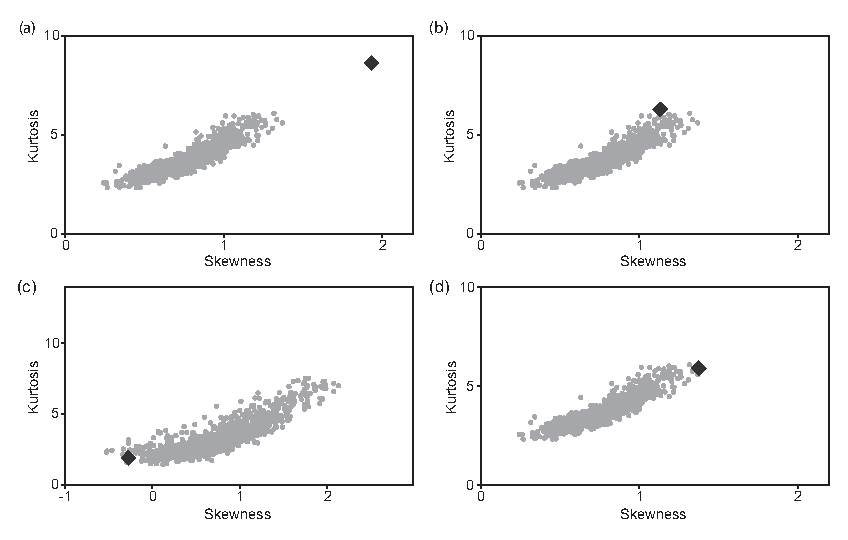
\includegraphics[width=0.5\linewidth]{\FigPath/fig4.eps}
\caption[Plots of skewness vs. kurtosis values for 95\% of 1000 simulated Poisson spatial distributions]{Plots of skewness vs. kurtosis values for 95\% of 1000 simulated Poisson spatial distributions. Diamonds represent the corresponding experimental values for a) all cataloged vents on Syria Planum, b) vents in both shield fields, c) vents in the northern shield field, and d) vents in the southern shield field. Randomness is rejected for all vents and for the combined shield fields (a, b respectively) at the 0.05 significance interval and accepted for both shield fields (c,d) individually. Simulated Poisson spatial distributions for a, b, and d use 300 data points; for c, 30 data points.}
\label{fig-skgraphs}
\end{figure}

All cataloged vents in the study area are first analyzed as a single group to test the null hypothesis, $H_o$, that the vents are spatially random in a Poisson sense. Spatial randomness of the entire study area could be evidence that a single magma production event may explain all volcanism in Syria Planum. However, due to the low $R$--index, the low $c$ statistic, and the result of the skewness/kurtosis test where the field plotted outside the range of Poisson randomness at the 99\% confidence interval, we reject the null hypothesis that the vents on Syria Planum are consistent with a Poisson spatial distribution when the entire study area is considered. Moreover, the observed $R$--index indicates that for all of Syria Planum the vents have a tendency to cluster, which is evidence that multiple subgroups might be identified as independent magma production events.

A subgroup that includes vents in both the northern and southern shield fields is also examined. Nearest neighbor results of this subgroup (N \& S row in Table \ref{tab-nn}) inconclusively characterize the randomness of the combined field. The observed $c$ statistic is within the predicted range, the $R$--index is calculated to be at the limit (\textit{R} = 1.11) of the expected $R \pm 2\sigma$, and the skewness and kurtosis values deviate from the elliptical centroid enough to reject randomness at the 0.05 significance level.

The vents within the northern shield field and the southern shield field are also analyzed individually to test their spatial randomness (Table \ref{tab-nn}). According to all three tests (the $R$--index, the $c$ statistic, and the skewness/kurtosis test) both the northern shield field and the southern shield field are found to exhibit Poisson spatial randomness individually. Therefore the null hypothesis of spatial randomness cannot be precluded for these shield fields. It is important to note that the northern shield field includes only 22 vents, increasing uncertainty in this conclusion. However, as the  southern shield field (n = 192) clearly exhibits spatial randomness and the combination of the two shield fields produces an ambiguous spatial distribution, there is evidence to suggest that the two shield fields are statistically distinct.

\subsection{Two--point azimuthal analysis}


\begin{figure}
\centering
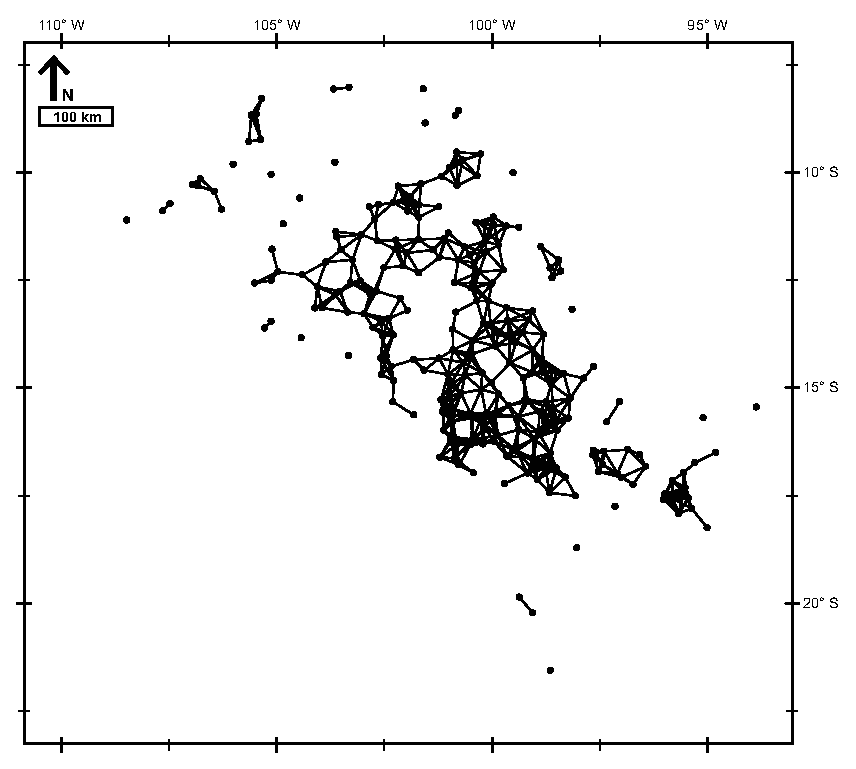
\includegraphics[width=0.5\linewidth]{\FigPath/fig5.eps}
\caption{Plot of vents and all inter--vent relationships less than the minimum significant distance.}
\label{fig-azmap}
\end{figure}

Figure \ref{fig-azgraphs}a displays a histogram of the lengths of all 34,453 inter--vent relationships. The skewness of this set of distances is 0.79. The mean distance, $\mu$, is 267~km and the standard deviation, $\sigma$, is calculated to be 157~km. The relationships used to investigate lineaments are below the minimum significant distance of $\le$~36.9~km as defined in Equation \ref{eq5} \citep{Cebria2011}. The number of inter--vent relationships, n, below the minimum significant distance, is 745. Figure \ref{fig-azmap} is a diagram of the vents represented as points in two-dimensional Cartesian space, using their locations in meters, and relationships between vents that are below the minimum significant distance.


\begin{figure}
\centering
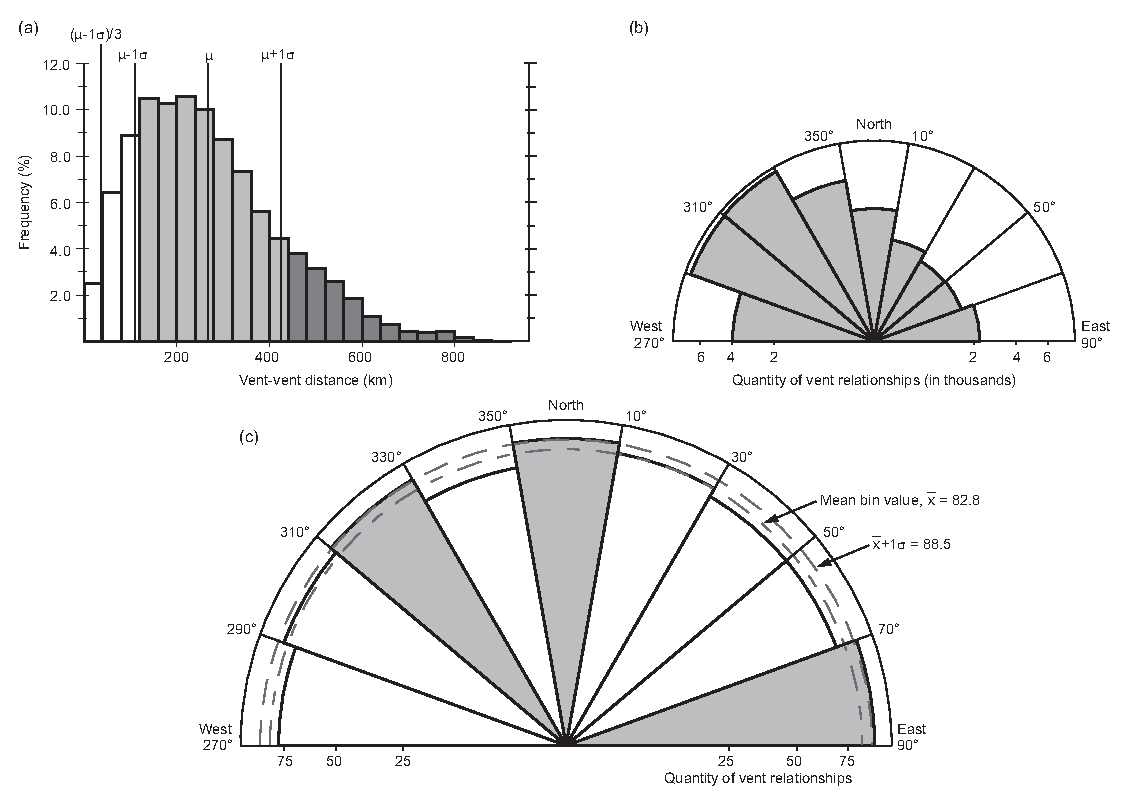
\includegraphics[width=0.7\linewidth]{\FigPath/fig6.eps}
\caption[Distribution of inter--vent distances and inter--vent alignments]{a) Distribution of inter--vent distances. Azimuths of inter--vent relationships are used if the inter--vent distance is less than 39.6 km, the defined minimum significant distance. Distances shaded dark gray are anomalously long and might trend in the overall vent field. Distances shaded light gray are of moderate length and are considered to be background noise. b) Directional distribution considering all inter--vent relationships. The plotted northwest mode is a result of including long distance inter--vent relationships. c) Direction distribution of inter--vent alignments below the minimum significant distance. The inner dotted line represents the mean quantity of inter--vent relationships. The outer dotted line represents the quantity of relationships one standard deviation above the mean. Directional wedges shaded gray (70-90$^{\circ}$, 310-330$^{\circ}$, 350-10$^{\circ}$) have anomalously high quantities of inter--vent relationships.}
\label{fig-azgraphs}
\end{figure}

The rose diagram in Figure \ref{fig-azgraphs}c illustrates the results of categorizing relationships based on the direction. The mean quantity of relationships in each direction bin, $\bar{x}_n$, is 82.8 and the standard deviation, $\sigma_n$, is 5.74. Three bins are identified as containing heightened amounts (count $\ge \bar{x}_n + \sigma_n$) of inter--vent relationships: 70-90$^{\circ}$ ENE, 350-10$^{\circ}$ N, and 310-330$^{\circ}$ NW.

A rose diagram (Figure \ref{fig-azgraphs}b) has been included, which illustrates the 2--point azimuth technique as applied to all inter--vent relationships, including those above the minimum significant distance. The NW trend of the relationships is comparable to the NW trend of the overall vent field.

\section{Discussion}

Previous analyses of post-\textit{Viking} era data show that the development of the Syria Planum region can be subdivided into a series of tectonic and volcanic episodes. The goal of this study is to provide additional detail to this sequence of events, and to determine if this region experienced one long--lived magmatic event or a series of magma production events. Building upon the work of \citet{baptista2008swarm} we present the following sequential volcano--tectonic development for the Syria Planum region based on superposition relationships. 1) Lava flows erupted from Syria Mons during the Early Hesperian (3.4-3.5 Ga), covering a recently (within hundreds millions of years) formed graben--rich basement unit. 2) Northeast faulting cross-cut the Syria Mons flows. 3) At 3.3-3.4 Ga during the Hesperian a southern shield field formed through the eruption of small volcanic vents in central Syria Planum to the NE of Syria Mons, which occurred contemporaneous to northwest faulting in the region of the vent field. 4) Volcanism continued throughout the northern region of Syria Planum from the Late Hesperian to the Early Amazonian (2.9-3.3 Ga), while concentrating to create a northeast trending ridge of coalesced vents north of and embaying the low shields of the southern shield field.

The most noticeable addition to the work of \citet{baptista2008swarm} is the separation of their coalesced shield field into a northern and southern coalesced vent field for which the northern is younger based on superposition. The delineation of two distinguishable vent fields in Syria, along with the development of Syria Mons, reveals at least three significant volcanic units or episodes. If these volcanic episodes all result from one magma production event then they display a migration and evolution in eruptive style as Syria volcanic units were emplaced through time. If not, then at least two, possibly more, magma production events produced the current surface of Syria Planum and should be considered in models of the overall development of the Tharsis province.

Crater counts of the units in this study (Table \ref{tab-crater}) are consistent with the inferred relative ages of the units based on superposition as presented above. Crater retention ages (Figure \ref{fig-unitages}) suggest that currently preserved lavas flowed across the Syria region as early as the Early Hesperian within the Syria Mons unit and last flowed as recently as the Late Amazonian during emplacement of the north field. We identify a slightly longer temporal range for volcanism at Syria than \citet{plescia2004morphometric} and \citet{baptista2008swarm} possibly due to our expanded mapping area and use of a more complete higher resolution set of data. Regardless, our results indicate that volcanism at Syria likely spanned a period of time no longer than $\sim$900 Ma. However, we also note that \citet{hauber2011very} conducted crater counts of select individual vents within Syria Planum, finding that some small shields might have erupted as recently as several hundred million years ago. Although our crater counts do not suggest significant temporal overlaps between the volcanic units, error bars do terminate against one another. As such, crater counts confirm our sequential inferences, but are inconclusive, taken on their own, with regard to differentiating between multiple and a single magma production event related to the emplacement of Syria Planum lava flows. 

The application of spatial and alignment statistical analyses to vent location data within monogenetic vent fields on the Earth have previously enabled researchers to identify unique vent populations within a field and their relationships to regional tectonics \citep[e.g.]{Connor2000}. Although such results are often supported by extensive field work, \citet{Bishop2007} showed the value of conducting such analyses based on remote sensing data alone, and recently researchers have demonstrated the potential for using those analyses on martian vent fields \citep{Bishop2008,bleacher2009spatial,Hamilton2010,Hamilton2011}. The Nearest Neighbor and 2--Point Azimuth analyses used here are based on decades of terrestrial research supported by field work and are used here to provide additional insight into the development of Syria Planum where mapping and crater counting alone cannot adequately test our hypothesis. 

\citet{Lutz1986} and \citet{lutz1995improved} suggest that vent fields with nonrandom spatial distributions represent an overlap of more than one population of randomly spaced vents. Nearest Neighbor analyses for the entire Syria Planum vent field yields a non-random spatial distribution of vents. Based on our mapping that delineates a northern and southern shield field in Syria Planum, and the work of \citet{Lutz1986} and \citet{lutz1995improved}, we interpret this result to indicate that at least two populations of vents with unique spatial signatures make up the Syria Planum region. Together, the vents of these fields yield a nearest neighbor result of questionable consistency with a random Poisson distribution, but removal of the northern field from the southern field yields a result clearly consistent with a random Poisson distribution for the southern field (Table \ref{tab-nn}). As such, our geologic interpretation of the random statistical spacing of these features is that the southern shield field represents one unique population of volcanic vents. The spacing of 22 vents in the northern shield field is also consistent with a random distribution. One interpretation of these Nearest Neighbor results is the existence of more than one magma production event, each identified by a randomly sorted population of vents in the study area. Another interpretation of Syria's overall nonrandom vent spacing is that magmatic activity migrated towards the north where magma ascension might have been controlled by different tectonic influences that affected the spacing dynamics of the subsequently emplaced vent field. The Nearest Neighbor results are consistent with the possibility of more than one magma production event, in contrast with age-dating results, which do not identify any detectable hiatus in eruptive activity during the entirety of the observable volcanic history of Syria Planum. In spite of this contrast, we are able to confidently state that the southern field is representative of a significant magma production event.The addition of the northern field vents to the southern field vents confuses those results: a clear distinction between two magma production events (southern \textit{and} northern) and a single evolving event (southern \textit{to} northern) is not found.

Many terrestrial volcanic fields display migrations in activity throughout the eruptive cycle associated with a major magma production event.  The Springerville Volcanic Field, AZ, is perhaps one of the best examples of this process. Monogenetic volcanism of Springerville was active from Late Pliocene to Holocene (2.1 to 0.3 Ma), producing basaltic low shields and cinder cones. Over the course of its volcanic activity, vent formation migrated eastward by roughly 2.5 cm/yr. A compositional progression is also seen: volcanism erupted tholeiitic basalts early on and changed over time to erupt alkalic olivine basalts \citep{condit1989patterns,Condit1999}.

The results of two--point azimuth analysis for Syria reveal three predominant trends of vent alignment centered at 0$^{\circ}$, 80$^{\circ}$, and 320$^{\circ}$ from north (Figure~\ref{fig-azgraphs}). We interpret the geologic cause of these alignments to be shallow faulting which constrained the placement of small vents. Most clearly, northwest faulting first observed by \citet{baptista2008swarm} occurred contemporaneously to the formation of the south field, which corresponds to the observed northwest vent alignment. Additionally, while the faulting pattern in the graben-rich basement unit trends NW, specifically trending between 330-350$^{\circ}$ which corresponds to a paucity of inter--vent alignments (Figure~\ref{fig-azgraphs}), it is possible that faulting continues and shifts direction where this basement unit is buried. East--west trending graben are observed in the northwest region of the study area extending from the western margins of Noctis Labyrinthus towards the northern shield field, which might correspond to the vent alignments observed at 80$^{\circ}$. Such a tectonic influence on magma ascension later in the development of the Syria Planum, particularly in the north, might have caused the confused Nearest Neighbor results discussed above. The alignment of vents to the north is not supported by faulting that is observable at the surface. This might provide insight into the possibility of buried regional--scale faults with north--south alignments.

This mapping project enables insight into the origin of Syria Mons and its relationship to the coalesced field of shields to the east and north.  The mapping presented here and by \citet{baptista2008swarm} demonstrates that Syria Mons is comparable to other large Tharsis shield volcanoes in areal extent, although with a much lower relief than Olympus Mons and the Tharsis Montes.  Does Syria Mons itself represent a unique magma production event that is distinct from the coalesced shields?  Superposition demonstrates a consistent embayment of Syria Mons by flows associated with the coalesced vent field.  However, crater count data again cannot be used to rule out the possibility of synchronous eruptions within these two units as their error bars end against each other. It is not uncommon for terrestrial shield volcanoes to experience a dispersal of eruption sites in the late stages of volcano growth.  This is perhaps best observed at Mauna Kea, Hawaii.  As Hawaiian shield volcanoes transition from the tholeiitic shield building to alkali capping stages the eruptions become less frequent and produce shorter flows \citep{Moore2007,Wolfe1996,Rowland2000,Bleacher2008}.  This transition is the result of numerous effects primarily related to a decrease in magma delivery rate to the surface as the volcano is pulled away from the consistently active Hawaiian hotspot due to plate tectonics.  This decrease in magma supply is no longer capable of sustaining a primary shallow magma reservoir at the older volcanoes like occurs at Kilauea or Mauna Loa, and as a result each eruption represents an isolated package of magma.  Because these eruptions do not share a shallow magma source they each find their own way to the surface and the eruption sites are dispersed across the volcano. Like the decreased magma supply rate at Mauna Kea, a decrease in the magma supply rate under Syria Mons might have caused a similar dispersal of eruption sites from one central vent volcano to a series of independent vents. Coupled with changing regional stress fields that are displayed by different fault orientations throughout Syria Planum, it might be possible for one major magma production event under the Syria region to have evolved from a sustained central vent edifice (Syria Mons) to plains--style, coalesced vent field volcanism that itself migrated from the southeast to northwest of Syria.  

\begin{figure}[ht]
\centering
\includegraphics[width=0.7\linewidth]{\FigPath/fig7.eps}
\caption[Map of tectonic centers from \citet{Anderson2001}]{\citet{Anderson2001} described tectonic centers located at numbered circles: 1) between Syria and Claritas Fossae in the Noachian, 2) along the southern-central portion of Valles Marineris in the Late Noachian and Early Hesperian, and 3) northwest of Syria into the Early Hesperian. Black circles: vents in this study; star: Syria Mons. The rose diagram of Figure 6c is reproduced in the bottom right to illustrate similarities between inter--vent alignments and directions between Syria Planum and tectonic centers.}
\label{fig-andersoncenters}
\end{figure}

Comparison of the vent spatial and alignment data with the tectonic history of the region yields additional insight into the sequential development of Syria. Syria Planum, and the surrounding areas, are identified as long standing centers of tectonic activity with major tectonic centers existing 1) between Syria and Claritas Fossae in the Noachian, 2) along the southern--central portion of Valles Marineris in the Late Noachian and Early Hesperian, and 3) northwest of Syria into the Early Hesperian \citep{Dohm1999,Anderson2001,Anderson2004} (See Figure \ref{fig-andersoncenters}).  \citet{Dohm1999} suggest that these tectonic centers likely resulted from significant volcano--tectonic activity, and likely produced much of the volcanic deposition that is seen in those regions today. Some of the regional (hundreds to thousands of kilometers) graben structures crossing Syria Planum described by \citet{Dohm1999}, have previously been described as having been utilized as dike pathways subsequent to formation in the Syria and neighboring Thumasia Regions \citep{Plescia1982,mege1996plume,Wilson2002}.

Comparison of our detailed analyses of the volcanic features within Syria to the tectonic evolution of Tharsis highlights some unique commonalities.  The tectonic history suggests a change in location and decrease in intensity of tectonic activity towards the northeast across the Syria region from Claritas Fossae to Valles Marineris, then westward across the northern extent of the Syria region between the Noachian and Early Hesperian \citep{Dohm1999,Anderson2002,Anderson2004}.  Volcanism in Syria, as revealed in this study, migrated east away from Syria Mons, and subsequently to the northwest between Early Hesperian and Early Amazonian. This migration was coupled with an evolution from one major central vent volcano, to broadly distributed volcanism that formed many, smaller central vent volcanoes whose flow fields coalesced to completely resurface Syria.  This style of volcanic evolution (single central vent to broadly distributed vents) is also associated, at least in part, with a waning magma supply on some terrestrial volcanoes \citep{Moore2007,Wolfe1996,Rowland2000,Bleacher2008}.  It is not clear at what time Syria Mons volcanism began.  \citet{Dohm1999} suggest that Noachian volcanism from the Syria region emplaced some of the basement units that were later deformed during the formation of Claritas Fossae and \citet{Webb2001} suggest that these eruptions built up the Syria Planum topographic rise by the Late Noachian to Early Hesperian as a major volcanic center that was $>$ 2000~km in diameter and displaying at least 8~km of relief.

A coupled tectonic history of Tharsis and volcanic evolution of Syria is presented here.  During the Noachian a center of province-wide tectonism was located between Syria and Claritas Fossae, essentially south of the study area. At this time extensive volcanic plains units were emplaced between Syria and the Thaumasia region to the south, for which no known vents are currently exposed at the surface in Syria. Tectonism at this time would have created radial crustal fractures that trended north through the study area, which is one of three orientations of heightened inter--vent relationships identified in the two--point azimuth analysis (Figure \ref{fig-azgraphs}). Between the Late Noachian and Early Hesperian the center of Tharsis tectonism shifted northeastward towards Valles Marineris.  At the same time volcanism in Syria evolved into a single central vent volcano, Syria Mons, although we cannot rule out the possibility of additional distributed volcanic centers across Syria that are now covered by younger deposits. At this time the tectonic center was located to the east of Syria and would have created west trending crustal structures through the study area, which again is an orientation of heightened inter--vent relationships in Syria (Figure \ref{fig-azgraphs}). During the Early Hesperian, as tectonism continued to shift, now towards the west/northwest, volcanism evolved into dispersed development of numerous small volcanic centers that were distributed across several hundred kilometers of the Syria region.  Tectonism related to this center would have created southeast trending crustal structures across the study area at this time, which is the orientation of the third heightened inter--vent relationship orientations identified in this study (Figure \ref{fig-azgraphs}).  Following the Early Hesperian, tectonism was focused far to the north near Alba Patera. Volcanism in Syria declined through the Hesperian and eventually ended sometime in the Early Amazonian.

\section{Conclusion}
Mapping of the Syria Planum region of Mars shows at least 263 volcanic vents ranging in diameter from one volcano $>$100~km (Syria Mons) to most volcanoes at 10s of km. Mapping, crater counts, and spatial and alignment statistical analyses reveal a complex volcano--tectonic history for this region that represents at least one major magma production event in the developmental history of Tharsis. 

Mapping of lava flows and vents, and their superposition relationships shows a sequence of volcanic activity from a broad shield volcano, Syria Mons, in the early Hesperian to a coalesced field of individually, areally smaller shields that together resurfaced much of the region through the Late Hesperian, possibly including the shields in northwest Syria.  This broadly distributed activity eventually became focused to form a northeast trending topographic ridge composed of the region's youngest group of small shield volcanoes into the Early Amazonian. Crater counts support these mapping--based inferences, indicating that each stage of activity followed the previous stage with no significant hiatus and that each stage likely lasted between 60 and 650~Ma. Spatial statistics are inconclusive with regard to differentiating multiple events, but do suggest that the earlier coalesced shield field and the northern ridge shield field each represent a unique randomly distributed group of vents. We interpret this result to indicate that each group's vents formed by the ascension and eruption of isolated magma bodies and did not share a common shallow magma reservoir for which magma scavenging of shared resources might have affected vent location.

Results from the study of Syria Planum tectonism and volcanism highlight the difficulty of identifying unique magma production events across planetary volcanic provinces for which detailed field work is not possible.  It is assumed that major shield volcanoes on Mars might be related to magma production events similar to the concept of mantle plumes in terrestrial geology. However, the cause of eruptions for shield field volcanism across such large areas of the Martian crust are more difficult to interpret. Our remote sensing--based mapping, crater counts, and spatial and alignment analyses do not conclusively demonstrate either that Syria experienced one, evolving magma production event, or a series of unique events that are spatially overlapping.  However, the tectonic evolution around and across Syria does demonstrate that the Syria region was influenced by evolving stress fields during the same timeframe that volcanic eruptions were occurring. We identify orientations of enhanced inter-vent alignments that are aligned with extensions of all three of the closest tectonic centers through our study area.  Although buried, these structural features within the underlying crust of Syria appear to have influenced the ascension of magma bodies to the surface between the Early Hesperian and Early Amazonian, as is seen for the field of volcanic vents south of Pavonis Mons \citep{bleacher2009spatial}.

It is clear that the Syria Planum region is a major center of Tharsis volcanism, and that this volcanic center is surrounded by at least three major tectonic centers, which appear to have influenced the locations of vent formation across Syria. The mapped distribution (both spatially and temporally) of volcanism in the region can be used to provide direct constraints for testing various hypotheses of the internal processes such as geodynamical models of melt generation from mantle convection \citep[e.g.]{ONeill2007} and/or lithospheric delamination \citep[e.g.]{Scott2003}. Although we cannot identify unique volcanic stages that are temporally isolated by eruptive hiatuses, we do identify the development of two unique units of coalesced small shields. The emplacement of these two shield fields occurred over a period of 100--800~Ma, both following the development of a major central vent volcano. When taken as a whole, the entire region evolved from a central--vent volcano to dispersed volcanism across $\sim$900~Ma. Our future work focuses on determining the volumes of lava erupted during these volcanic events as an additional modeling constraint. Continued mapping of surface features should provide direct constraints for future integrated geodynamic models of volcanic and tectonic processes that were related to significant Tharsis province magma production events.

\begin{table}[h]
\caption{Notation}
\centering
\begin{tabular}{r p{7cm}}
\toprule
  $c$&test statistic for spatial randomness.\\
  $\bar{r}_a$&observed mean Nearest Neighbor distance.\\
  $\bar{r}_e$&expected mean Nearest Neighbor distance.\\
  $\sigma_e$&expected standard deviation of Nearest Neighbor distances.\\
  $R$&index comparing $\bar{r}_a$ and $\bar{r}_e$ to test spatial randomness.\\
  $d$&minimum significant distance of 2-point azimuth analysis.\\
  $\mu_v$&mean inter--vent distance.\\
  $\sigma_v$&standard deviation of inter--vent distances.\\
  $\bar{x}_n$&mean quantity of inter--vent relationships in directional bins.\\
  $\sigma_n$&standard deviation of inter--vent relationships in directional bins.\\
\bottomrule
\end{tabular}
\label{tab-notation}
\end{table}

\section{Acknowledgments}

Funding for this project was provided to all three authors by NASA's Mars Data Analysis Program. Additional support for J. Richardson was provided by NASA's Undergraduate Student Research Program funding through Goddard Space Flight Center. We thank Nick Schmerr for insightful comments that improved the content of this report.

%%%%%%%%%%%%%%%%%%%%%%%%%%%%%%%%
%References
%%%%%%%%%%%%%%%%%%%%%%%%%%%%%%%%

\section{References}
% authors generating their own bbl file would uncomment the following two lines, and comment out/delete the references below:
\bibliography{dissertation_refs}% reads igs2eguide.bib
\bibliographystyle{apalike}  % imposes IGS bibliography style on output

